% !BIB TS-program = biber

\RequirePackage[l2tabu,orthodox]{nag}

% TODO: decide if one-sided/two-sided
%\documentclass[headsepline,footsepline,footinclude=false,fontsize=11pt,paper=a4,listof=totoc,bibliography=totoc,BCOR=12mm,DIV=12]{scrbook} % two-sided
\documentclass[headsepline,footsepline=false,footinclude=false,oneside,fontsize=11pt,paper=a4,listof=totoc,bibliography=totoc]{scrbook} % one-sided

% TODO: change citation style in settings
\PassOptionsToPackage{table,svgnames,dvipsnames}{xcolor}

\usepackage[utf8]{inputenc}
\usepackage[T1]{fontenc}
\usepackage[sc]{mathpazo}
\usepackage[ngerman,american]{babel}
\usepackage[autostyle]{csquotes}
\usepackage[%
  backend=biber,
  url=false,
  style=authoryear,
  maxnames=4,
  minnames=3,
  maxbibnames=99,
  giveninits,
  uniquename=init]{biblatex} % TODO: adapt citation style
\usepackage{graphicx}
\usepackage{svg}
\usepackage{scrhack} % necessary for listings package
\usepackage{listings}
\usepackage{lstautogobble}
\usepackage{tikz}
\usepackage{pgfplots}
\usepackage{pgfplotstable}
\usepackage{booktabs}
\usepackage[final]{microtype}
\usepackage{caption}
\usepackage{subcaption}
\usepackage[hidelinks]{hyperref} % hidelinks removes colored boxes around references and links
\AtBeginDocument{%
  \hypersetup{
    pdftitle=\getTitle,
    pdfauthor=\getAuthor,
  }
}

\usepackage[acronym,xindy,toc]{glossaries}
\makenoidxglossaries

\usepackage{geometry}
\geometry{
  inner=30mm,
  outer=26mm,
  top=30mm,
  bottom=30mm,
  heightrounded,
  marginparwidth=51pt,
  marginparsep=17pt,
  headsep=24pt,
}

\usepackage{ifthen}

\usepackage{multirow}

\addto\extrasamerican{
  \def\lstnumberautorefname{Line}
  \def\chapterautorefname{Chapter}
  \def\sectionautorefname{Section}
  \def\subsectionautorefname{Subsection}
  \def\subsubsectionautorefname{Subsubsection}
}

\addto\extrasngerman{
  \def\lstnumberautorefname{Zeile}
}

% Themes
\ifthenelse{\equal{\detokenize{dark}}{\jobname}}{%
  % Dark theme
  \newcommand{\bg}{black} % background
  \newcommand{\fg}{white} % foreground
  \usepackage[pagecolor=\bg]{pagecolor}
  \color{\fg}
}{%
  % Light theme
  \newcommand{\bg}{white} % background
  \newcommand{\fg}{black} % foreground
}

\bibliography{meta/bibliography}

\setkomafont{disposition}{\normalfont\bfseries} % use serif font for headings
\linespread{1.05} % adjust line spread for mathpazo font

%\setmainfont{font/TUMNeueHelvetica-Regular.ttf}[
%  BoldFont       = TUMNeueHelvetica-Bold.ttf ,
%  ItalicFont     = TUMNeueHelvetica-Italic.ttf ,
% BoldItalicFont = TUMNeueHelvetica-BoldItalic.ttf]

% Add table of contents to PDF bookmarks
\BeforeTOCHead[toc]{{\cleardoublepage\pdfbookmark[0]{\contentsname}{toc}}}

% Define TUM corporate design colors
% Taken from http://portal.mytum.de/corporatedesign/index_print/vorlagen/index_farben
\definecolor{TUMBlue}{HTML}{0065BD}
\definecolor{TUMSecondaryBlue}{HTML}{005293}
\definecolor{TUMSecondaryBlue2}{HTML}{003359}
\definecolor{TUMBlack}{HTML}{000000}
\definecolor{TUMWhite}{HTML}{FFFFFF}
\definecolor{TUMDarkGray}{HTML}{333333}
\definecolor{TUMGray}{HTML}{808080}
\definecolor{TUMLightGray}{HTML}{CCCCC6}
\definecolor{TUMAccentGray}{HTML}{DAD7CB}
\definecolor{TUMAccentOrange}{HTML}{E37222}
\definecolor{TUMAccentGreen}{HTML}{A2AD00}
\definecolor{TUMAccentLightBlue}{HTML}{98C6EA}
\definecolor{TUMAccentBlue}{HTML}{64A0C8}

% Settings for pgfplots
\pgfplotsset{compat=newest}
\pgfplotsset{
  % For available color names, see http://www.latextemplates.com/svgnames-colors
  cycle list={TUMBlue\\TUMAccentOrange\\TUMAccentGreen\\TUMSecondaryBlue2\\TUMDarkGray\\},
}

% Settings for lstlistings
\lstset{%
  basicstyle=\ttfamily,
  columns=fullflexible,
  autogobble,
  keywordstyle=\bfseries\color{TUMBlue},
  stringstyle=\color{TUMAccentGreen},
  captionpos=b
}

\newacronym{VAE}{VAE}{variational autoencoder}
\newacronym{GHG}{GHG}{greenhouse gas}
\newacronym{DWT}{DWT}{discrete wavelet transform}
\newacronym{DCT}{DCT}{discrete cosine transform}
\newacronym{Lasso}{Lasso}{least absolute shrinkage and selection operator}
\newacronym{BP}{BP}{basis pursuit}
\newacronym{BPDN}{BPDN}{basis pursuit with denoising}
\newacronym{LS}{LS}{regularized least squares}
\newacronym{GAN}{GAN}{generative adversarial network}
\newacronym{RIP}{RIP}{restricted isometry property}
\newacronym{KL}{KL}{Kullback-Leibler}
\newacronym{ELBO}{ELBO}{evidence lower bound}
\newacronym{MSE}{MSE}{mean squared error}
\newacronym{SSIM}{SSIM}{structural similarity index}
\newacronym{RE}{RE}{relative error}
\newacronym{MCMC}{MCMC}{Markov Chain Monte Carlo}
\newacronym{MAP}{MAP}{maximum a posteriori}
\newacronym{SNR}{SNR}{signal to noise ratio}
\newacronym{SP}{SP}{signal power}
\newacronym{ResConv}{ResConv}{residual convolutional layers}

% refer to https://en.wikibooks.org/wiki/LaTeX/Glossary for acronyms and glossary entries
% \newglossaryentry{gamma}
% {
%   name={\ensuremath{\gamma}},
%   description={Regularization factor in generative model solver},
%   sort=gamma
% }

% \newglossaryentry{lambda}
% {
%   name={\ensuremath{\lambda}},
%   description={Regularization factor in sparse generative model solver},
%   sort=lambda
% }



% TODO: change thesis information
\newcommand*{\getUniversity}{Technische Universität München}
\newcommand*{\getChair}{Professorship of Environmental Sensing and Modeling}
\newcommand*{\getDepartment}{Department of Electrical Engineering}
\newcommand*{\getSchool}{Computation, Information and Technology}
\newcommand*{\getTitle}{Learning Compressed Representations of Emission Inventories in Urban Environments}
\newcommand*{\getTitleGer}{Erlernen komprimierter Darstellungen von Emissionen in städtischen Umgebungen}
\newcommand*{\getAuthor}{Mustafë Dobra}
\newcommand*{\getDoctype}{Master's Thesis}
\newcommand*{\getAdvisor}{Moritz Makowski}
\newcommand*{\getExaminer}{Prof. Dr.-Ing. Jia Chen}
\newcommand*{\getSubmissionDate}{13.11.2024}
\newcommand*{\getSubmissionLocation}{Munich}

% Macros
\newcommand{\norm}[1]{\left\lVert#1\right\rVert}

\begin{document}

% Set page numbering to avoid "destination with the same identifier has been already used" warning for cover page.
% (see https://en.wikibooks.org/wiki/LaTeX/Hyperlinks#Problems_with_Links_and_Pages).
\pagenumbering{alph}
\begin{titlepage}
    % HACK for two-sided documents: ignore binding correction for cover page.
    % Adapted from Markus Kohm's KOMA-Script titlepage=firstiscover handling.
    % See http://mirrors.ctan.org/macros/latex/contrib/koma-script/scrkernel-title.dtx,
    % \maketitle macro.
    \oddsidemargin=\evensidemargin\relax
    \textwidth=\dimexpr\paperwidth-2\evensidemargin-2in\relax
    \hsize=\textwidth\relax

    \centering

    \vspace*{5mm}

    \IfFileExists{template/logos/tum-logo-blue.png}{%
        
\includegraphics[height=20mm]{template/logos/tum-logo-blue.png}
    }{%
        \vspace*{20mm}
    }

    \vspace{20mm}

    {\huge\MakeUppercase{TUM School of \getSchool{}} \par}

    \vspace{5mm}
    {\large\MakeUppercase{\getDepartment{}} \par}

    {\large\MakeUppercase{\getChair{}} \par}

    \vspace{15mm}

    {\huge\bfseries \getTitle{} \par}

    \vspace{10mm}
    {\LARGE \getAuthor{}}

\end{titlepage}




\frontmatter{}

\begin{titlepage}
    \centering

    \vspace*{5mm}

    \IfFileExists{template/logos/tum-logo-blue.png}{%
        
\includegraphics[height=20mm]{template/logos/tum-logo-blue.png}
    }{%
        \vspace*{20mm}
    }

    \vspace{20mm}
    {\huge\MakeUppercase{School of \getSchool{}} \par}

    \vspace{5mm}
    {\large\MakeUppercase{\getDepartment{}} \par}

    {\large\MakeUppercase{\getChair{}} \par}

    \vspace{20mm}

    {\huge\bfseries \getTitle{} \par}

    \vspace{10mm}
    {\huge\bfseries \foreignlanguage{ngerman}{\getTitleGer{}} \par}

    \vspace{15mm}

    \begin{tabular}{l l}
        Author:            & \getAuthor{}         \\
        Thesis Supervisor: & \getExaminer{}       \\
        Advisor:           & \getAdvisor{}        \\
        Submission Date:   & \getSubmissionDate{} \\
    \end{tabular}

    \vspace{25mm}
    \IfFileExists{template/logos/esm-logo-square.png}{%
        \vfill{}
        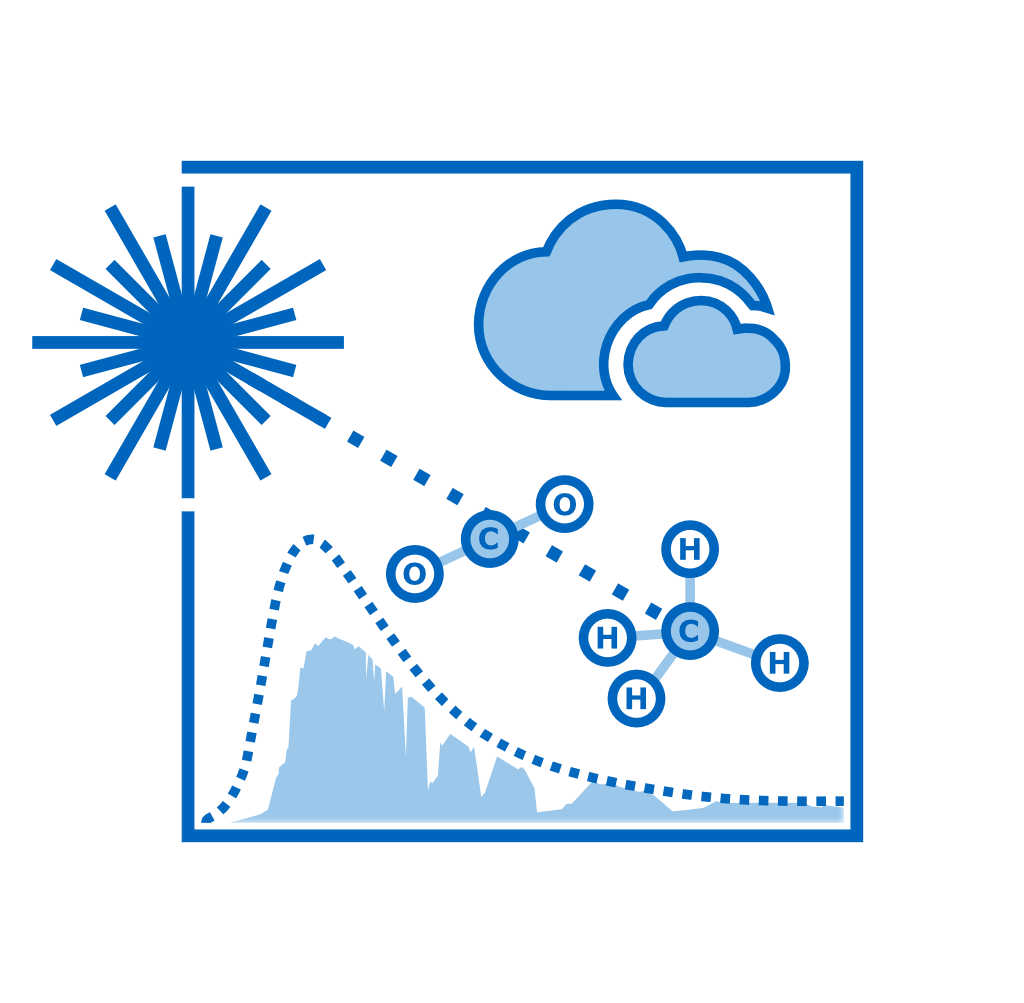
\includegraphics[height=20mm]{template/logos/esm-logo-square.png}
    }{}

\end{titlepage}

\thispagestyle{empty}
\vspace*{0.8\textheight}
\noindent
I confirm that this \MakeLowercase{\getDoctype{}} is my own work and I have documented all sources and material used.

\vspace{15mm}
\noindent
\getSubmissionLocation{}, \getSubmissionDate{} \hspace{50mm} \getAuthor{}

\cleardoublepage{}

\addcontentsline{toc}{chapter}{Acknowledgments}
\thispagestyle{empty}

\vspace*{20mm}

\begin{center}
    {\usekomafont{sectioning}\usekomafont{section} Acknowledgments}
\end{center}

\vspace{10mm}

Duis qui ea sint proident cillum sint sint culpa pariatur duis sunt commodo consequat reprehenderit. Officia sit veniam laborum aliqua. Minim reprehenderit consectetur laborum sint laboris quis et ullamco cillum adipisicing reprehenderit. Nostrud ullamco quis do ea cillum nostrud occaecat amet adipisicing aliqua aliquip.

\cleardoublepage{}

\chapter{\abstractname}

Global warming poses a significant challenge to our planet.
Emission Inventories have emerged as essential tools for climate mitigation.
However, they may be inaccurate, which motivates the need for inversion techniques that invert atmospheric transport using meteorological data and concentration measurements of greenhouse gases.
Typically, these inversion techniques require accurate priors.
Recent work has successfully investigated the applicability of compressed sensing in urban environments, alleviating the need for such priors.
This thesis builds on these approaches, investigating the applicability of compressed sensing techniques based on machine learning.
In particular, this thesis investigates an approach based on generative models.

A dataset of urban emission flux fields with a resolution of $1 \unit{km} \times 1 \unit{km}$ is built based on the high-resolution TNO-GHGco emission inventories from $2015$ and $2018$.
Three cities, Munich, Paris, and Zurich, are selected as case studies.
A variational autoencoder (VAE) is then trained on this dataset and evaluated on atmospheric inversion tasks, assuming that the largest emitters and background emissions are known. 

In particular, measurements are taken in simulated experiments with artificial footprints based on Gaussian plume simulations.
The reconstructions are evaluated based on relative error and SSIM and compared to a regularized least squares approach and sparse reconstruction algorithms using discrete cosine and discrete wavelet transforms.
Overall, the results show the competitive performance of the VAE with the approaches above for Munich and Zurich, while it fell short for Paris.
The VAE demonstrates a general strength in the structural similarity.

This thesis further experiments with modifications of the signal space the generator can generate, also called the range of the generator, by altering the latent dimension of the VAE and fine-tuning it to the case study cities.
These experiments reveal a trade-off between the size of the range and the search in that space, with a larger range decreasing the representational error; however, more information is required to find solutions.
The fine-tuned models improve the reconstruction performance significantly, beating the other approaches significantly for Munich and Zurich while closing the performance gap for Paris.
However, open work remains to investigate how these fine-tuned models deal with uncertainties in the inventories.

Finally, the generator is investigated in a controlled benchmark, revealing that this model does not fully capture the emission flux field distribution.
This limitation can likely be attributed to a need for more training data.

Overall, this thesis demonstrates that approaches based on machine learning are promising for urban emission flux reconstruction, with the potential for enhancement through more comprehensive urban datasets.


\clearpage

\glsnogroupskiptrue
\printnoidxglossaries

\clearpage

\microtypesetup{protrusion=false}
\tableofcontents{}
\microtypesetup{protrusion=true}

\mainmatter{}

% !TeX root = ../main.tex
% Add the above to each chapter to make compiling the PDF easier in some editors.

\chapter{Introduction}\label{chapter:introduction}

\begin{enumerate}
	\item Medical Imaging
	\item Global Warming
	\item Optional: Emission Inventories
	\item Area sources are not sparse and thus sparse reconstruction does not work well on them without transform
\end{enumerate}

\section{Motivation}
Bottom-up emission estimations are inaccurate.
Instead, top-down approaches could be used.
... et al. demonstrate that top-down approaches can be represented as an inverse problem with measurements $y$ and the emission field as $x$.
The transport of ghg molecules can be modeled as a linear map $A$ between $y$ and $x$, resulting in the following inverse problem:
\begin{equation}
	y = Ax
\end{equation}
In their paper, ... et al. show that using

Three reasons for bottom-up approach:
\begin{itemize}
	\item find unknown emitters
	\item determine diff. between bottom-up \& top-down
	\item find emitters not captured by inventories
\end{itemize}

\section{Research Questions}
This thesis aims at answering some questions:

\begin{itemize}
	\item How well can a variaional autoencoder capture a low dimensional representation of area sources in emission inventories?
	\item What is the effect of the dimension of that low dimensional space?
	\item Is the variational autoencoder generazible to all urban emission fields or should it be specialized on one city?
	\item How well does such a variational autoencoder perform in atmospheric inversion of area sources as a downstream task compared to state of the art approaches?
\end{itemize}

% !TeX root = ../main.tex
% Add the above to each chapter to make compiling the PDF easier in some editors.

\chapter{Related Work}\label{chapter:related_work}

\section{Compressed Sensing}
There are three main approaches to alleviate sparsity constraint.
1) transforms, such as Wavelet
2) only searching for unknown emissions and take esimtations as basis
3) Deep learning based approaches

\section{Deep Learning for Inverse Problems}
The field of medical imaging has made advancements in the inverse problems using deep learning.

\section{Generative Models}

\section{Contributions}

% !TeX root = ../main.tex
% Add the above to each chapter to make compiling the PDF easier in some editors.

\chapter{Methods}\label{chapter:methods}

\section{Dataset}
Datasets such as CAMS (cite) or TNO (cite) provide GHG emissions in a 0.1 times 0.05 lat times long resolution which corresponds to ~5 by ~5 kilometers.
This resolution is very low and urban data cannot effectively be extracted.
For instance, a city contained within a 30km by 30km grid, would contain 6 by 6 cells.
This is not enough to draw any meaningful information and conclusion. 
Therefore, this thesis focues on the high res $2015$ and $2018$ TNO datasets are used.
These are two high resolution, roughly 1km by 1km, emission inventory and thus high resolution emission fields in urban environments can be extracted.
The inventory contains GHG emissions for each GNFR sector (cite), with the road sector $F$ being split into $4$ sub sectors, for each coordinate in a defined grid within Europe.
This results in $15$ emission values per gas per cell.
For this thesis, only CO2 from fossil fuels are considered.
However, the presented approaches can be directly applied for all types of GHG sources.

\subsection{Urban Emission Fields}
Urban environments differ from non-urban environments in terms of their emissions.
For instance, urban environments often have a city center that generates a large portion of emissions as seen for example in Munich (picture of Munich).
Therefore, as the focus of this thesis are urban environments, they have to be filtered from the TNO datasets.
For this, a number of cities are selected from a public database by OpenDatasoft (cite here).
Cities are filtered according to their population size.
For this thesis, the population threshold is set to $100000$.
The resulting number of extracted cities is $2xx$.
A list of all cities with the corresponding coordinates is appended in the appendix.

From the filtered cities, the coordinates are used to extract emission fields.
From the TNO dataset, $n$ by $n$ grids around the city center are extracted.
This corresponds to a dimension of n km by n km.
While most cities are not even close to this size, this allows to later crop the fields to a desired size.
For this thesis, emission fields have $32$ by $32$.

The number of extracted emission fields is not enough to train a generative model.
Thus, temporal scaling factors from (cite) are used to generate more samples.
Scaling factors are applied to individual GNFR sectors.
This results in $24 * 7 * 12 = 2016$ samples per city per year.
The resulting dataset size is thus $2xx * 2 * 2016 = $ samples.
To reduce the memory overhead, scaling factors are applied at sampling time and only the original data is kept in memory.

\subsection{Dataset split}
The emission fields are split into training, validation, and test data.
The training data is used to train the model and updates its weights and makes up $\sim  70\%$ of the data.
The validation data is used to evaluate the generalization capabilities of the model during training and makes up $\sim  15\%$.
The test data is used for subsequent experiments and evaluations and makes up $\sim  15\%$.

For splitting, the emission fields are first sorted alphabetically by the city name.
Then, the first $15\%$ of cities are assigned to the test data.
This makes the split deterministic and thus reproducible.

The remaining cities are then randomly shuffled.
Finally, the first $\frac{0.15}{0.85}$ of cities are assigned to the validation set.
The remaining cities are assigned to the training set.

Maybe make a diagram here.

The number of samples in training, validation, and test set is given in table (make table).
A list of the cities in the test set is appended in appendix (add appendix).

\subsection{Data Augmentation}
To improve the generalization abilities of the model CITE, common image augmentation techniques are applied (to cite) to the emission fields in the training data.
First, random cropping is used.
Furthermore, a random horizontal flip and vertical flip are applied with probability $0.5$ each.
Lastly, emission fields are randomly rotated by 90$\circ$ with probability of $0.5$.
This results in $8$ different transformations, with one of them being the original emission field.

The validation and test emission fields are not transformed, except for a center crop.

\subsection{Scaling}
Scaling is an important factor for machine learning.
Large-scale data can make training converge slow and instable (cite).
Furthermore, regularization techniques such as batch normalization rely on scaled values (cite).
A common technique for scaling values is min max scaling (cite).
However, min max scaling is sensitive to outliers and thus not ideal for emission inventories where range of emissions within a city can largely differ.
Instead, robust scaling (cite) can be applied.
To determine a good scaling factor, the $95$th percentile of values is determined for each city in the training set.
The inverse of the average is then used as the scaling factor.
The resulting scaling factor is thus $\frac{1 a}{2.5 * 10^6 kg}$

\section{Variational Autoencoder}
The optimizer is AmsGrad (cite).
The architecture is inspired by (Walking the Tightrope: An Investigation of the Convolutional Autoencoder Bottleneck cite).
This means that the last layers before the fully connected layers has high width and height.
The encoder uses 2 2-stride layers to halve the width and height of the emission field, resulting in a width/height of 16 and 8 respectively.
The decoder makes use of tranpose conv layers to double the width/height of the emission field to get back to the original dimensions.
In between these conv layers that change the width and height, residual layers (cite) are used.
The conv layers in the residual layers have kernel size 2 and stride 1, thus retaining the width and height of the field when padding is used.
For activation, LeakyRelu (cite) is used except at the output of the residual layers where ReLu (cite) is used.
In addition, after every activation, except at the output of the residual layers, batch normalization (cite) is applied.
The exact architecture with channels and number of layers can be seen in Figure , created with the following GitHub Repository (https://github.com/HarisIqbal88/PlotNeuralNet?tab=readme-ov-file).

\subsection{Architecture}

\section{Evaluation}

\subsection{Gaussian Measurements}
In order to evaluate the generative capbailities in the context of inverse problems, a compressed sensing problem is used for evaluation.
This compressed sensing problem is based on the paper by Bora et al. as they mention that the performance of generative models can be assesed based on their provided problem statement.
For this, a identically independent distributed matrix $A \in R^{m \times 15000}$ is sampled for each run.
The following inverse problem is then solved using the minimization problem proposed by Bora et al.
\begin{equation}
    y = A x + \epsilon
\end{equation}
with $x$ being the emission fields $x^*$ in vectorized form.
This inverse problem is equivalnt to taking taking $m$ measurements that is randomly linearly affected by any sector in any cell within the emission field grid.
While this does not correspond to a typical transport model which follows the law of physics, this problem serves as a good proxy for evaluating the generative capbailities in the context of inverse problems of the trained VAE. 

The evaluation is performed on scaled emission fields.

The resulting pipeline is the following:
\begin{enumerate}
    \item Generate random A
    \item Sample x from test set
    \item Vectorize x
    \item Compute y from forward model
    \item Run reconstruction algorithm (minimization problem)
    \item Unvectorize resulting x dach
    \item Compare x with x dach
\end{enumerate}

Let $D$ be the decoder of the variational autoencoder.
Then, the generator $G: R^k \rightarrow R^{15000}$ can be written as $G(z) = \text{vec}(D(z))$, i.e. the generator G is the vectorization of the decoder of the VAE.

The minimization problem
\begin{equation}
    z^* = \arg\min_{z}{\norm{A G(z) - y} + R(z)}
\end{equation}
with $R(z) = \norm{z}$ is solved using the Adam Optimizer (cite).
For the learning rate, values are chosen based on the number of measurements, as seen in table (make table).
These values are determined empirically.

The reconstruction algorithm is run for the following number of measurements:
For each of the numbers, the reconstruction is run for each emission field in the test dataset.
A random measurement matrix $A$ is generated and each of the $3$ algorithms solve the same inverse problem.
The temporal transforms are disabled during evaluation which means that for each city only one emission field per year is used.
The evaluation is run 5 times to reduce randomness resulting from random initialization of $z$.

\subsection{Gaussian Plume Model}
Gaussian sensing matrix do not represent the real the emission problem well.
Instead of randomly samples sensing matrices, transport models should be used that indicate the sensitivity of measurements with resepect to physical grid cells based on the transport of molecules in the past.
These transport models are computationally expensive to compute and in generel difficult to estimate on a per city basis.
Thus, we apply the same idea as Benji in his work.
We substitue typical transport models, such as STILT, with a Gaussian plume model.
In his paper, Benji reconstructed the emission field without considering the indivudal sectors as contributors.
In this thesis, a full reconstruction is attempted, i.e. all $15$ sectors are reconstructed.
Therefore, the sensing matrix based on the Gaussian plume model must be adapted accordingly.

The forward model is the following:
\begin{equation}
    y = [A, \dots, A] [x_{s_0}, \dots, x_{s_{14}}]^T
\end{equation}
$A$ is the Gaussian plume model for n measurements.
$x_{s_i}$ is the emission field for a single sector.


% !TeX root = ../main.tex
% Add the above to each chapter to make compiling the PDF easier in some editors.

\chapter{Results}\label{chapter:results}

\section{Section}


% !TeX root = ../main.tex
% Add the above to each chapter to make compiling the PDF easier in some editors.

\chapter{Discussion}\label{chapter:discussion}

\section{Section}


% TODO: add more chapters here

\appendix{}

\microtypesetup{protrusion=false}

%\addchap{Abbreviations}
%\begin{acronym}
%\itemsep-.25\baselineskip
%\acro{TUM}[TUM]{Technical University of Munich}
% TODO: add acronyms
%\end{acronym}

\listoffigures{}
\listoftables{}
\microtypesetup{protrusion=true}
\printbibliography{}

\end{document}
